\chapter{Equilibrium Thermodynamics} \label{chap:equilibrium}

	The foundations of thermodynamic equilibrium calculations were laid down by American chemical physicist Josiah Willard Gibbs who originally published his work \emph{On the Equilibrium of Heterogeneous Substances} in a relatively obscure American journal, the Transactions of the Connecticut Academy of Arts and Sciences, in several parts, during the years 1875 to 1878. Thermodynamic equilibrium computations in isothermal, isobaric systems are aimed at identifying a unique combination of phases and species which minimises the integral Gibbs energy of the system while satisfying the necessary underlying conditions. Thermodynamics requires that a favourable change in a system must decrease the Gibbs energy of the system while respecting the mass constraints of the system components and the Gibbs' phase rule must be satisfied.

  \section{Conditions of thermodynamic equilibrium}\label{sec:eqb_theory}
		The law of \textbf{conservation of mass} requires that the linear equations representing mass constraints be satisfied. For component $j$, the mass balance equation can be written as
			\begin{equation}\label{eq:massbalance}
				b_j = \sum_{\lambda=1}^{\Lambda} n_{\lambda}\sum_{i=1}^{N_{\lambda}}x_{i({\lambda})}{\nu}_{i,j} +  \sum_{\omega=1}^{\Omega} n_{\omega}{\nu}_{\omega}
			\end{equation}
			where, ${\nu}_{i,j}$ and ${\nu}_{\omega}$ represent the stoichiometric coefficients of element $j$ in solution phase species $j$ and stoichiometric phase $\omega$ respectively. In an electrochemical system where the electrons form a system component with zero moles overall in the system, the mass balance constraint represents charge neutrality constraint.

		Thermodynamic equilibrium conditions also require that the \textbf{Gibbs' phase rule} must also be satisfied. Gibbs' phase rule determines the \emph{degree of freedom} of the system i.e. the number of phases that can be stable at equilibrium in relation to the state variables \cite{Gibbs:1878aa}. In general, the phase rule can be written as:
			\begin{equation}
                			F=C-\Phi + 2 + \Xi
            		\end{equation}
            		where, $F$ represents the degrees of freedom, $C$ denotes the number of components in the system, $\Phi$ denotes the number of phases and $\Xi$ denotes the number of ionic phases. However, for isothermal, isobaric systems with no charged species, the phase rule takes the following simplified form :
			\begin{equation}
                			F=C-\Phi
            		\end{equation}
			which implies that the number of phases that can co-exist at equilibrium cannot exceed the number of components in a closed isothermal, isobaric system.

		Ensuring that the Gibbs phase rule and mass balance constraints are satisfied is relatively straightforward but special attention must be paid to ensuring that the integral Gibbs energy of the system is at a minimum. The equilibrium criteria established by Gibbs requires that at equilibrium $d G_{sys} = 0$ \cite{Gibbs:1878aa}. Thus, differentiating equation~\ref{eqn:integralGibbs}
		\begin{equation}\label{eqn:dGibbs1}
			d G_{sys} = \sum_{\phi=1}^{\Phi} \sum_{i=1}^{N_{\phi}} \left( d n_{i(\phi)}\mu_{i(\phi)} + n_{i(\phi)} d \mu_{i(\phi)}\right) = 0
		\end{equation}

		The chemical potentials are related through the \emph{Gibbs-Duhem equation} which, at constant temperature and pressure, can be written as \cite{Olander08}:
		\begin{equation}\label{eqn:dGibbs2}
			\sum_{\phi=1}^{\Phi} \sum_{i=1}^{N_{\phi}} \left( n_{i(\phi)} d \mu_{i(\phi)}\right) = 0
		\end{equation}

		Substituting the Gibbs-Duhem equation in equation~\ref{eqn:dGibbs2} gives:
		\begin{equation}\label{eqn:dGibbs3}
			d G_{sys} = \sum_{\phi=1}^{\Phi} \sum_{i=1}^{N_{\phi}} \left( d n_{i(\phi)}\mu_{i(\phi)} \right) = 0
		\end{equation}

		The chemical potentials of the species can be written in terms of the chemical potentials of the system components. Therefore, substituting equation~\ref{eq:massbalance} into equation~\ref{eq:elempot}, differentiating with respect to $n_{i(\phi)}$ at constant temperature and pressure and equating to zero gives:
		\begin{equation}\label{eqn:dGibbs4}
			d G_{sys} = \sum_{\phi=1}^{\Phi} \sum_{i=1}^{N_{\phi}}  d n_{i(\phi)}\sum_{j=1}^{C}\nu_{i,j}\Gamma_j  = 0
		\end{equation}

		Rearranging gives:
		\begin{equation}\label{eqn:dGibbs5}
			\sum_{\phi=1}^{\Phi} \sum_{i=1}^{N_{\phi}}  d n_{i(\phi)} \left( \mu_{i(\phi)} - \sum_{j=1}^{C}\nu_{i,j}\Gamma_j \right) = 0
		\end{equation}

		Since both $\nu_{i,j}$ and $\mu_{i(\phi)}$ are unique for every species, the chemical potentials of species or phase in the system can be related to chemical potentials of system component at equilibrium through the following equation \cite{vanZeggeren11}:
		\begin{equation}\label{eqn:dGibbs6}
			\mu_{i(\phi)} = \sum_{j=1}^{C}\nu_{i,j}\Gamma_j
		\end{equation}

		Ensuring that equation~\ref{eqn:dGibbs6} is satisfied for all species in the system is equivalent to satisfying the equilibrium criterion that the Gibbs energy of the system is at a local minimum. This is useful in developing a convergence criterion for thermodynamic equilibrium calculations and is discussed in the following section.

	\section{Convergence criteria}
	A number of different methods can be proposed to judge the convergence of a thermodynamic equilibrium solver, the most obvious being ensuring that the relative change in Gibbs energy between two iterations is within a specified tolerance. Another approach that makes better use of principles of thermodynamic equilibrium is based on equation~\ref{eqn:dGibbs6} and requires that the chemical potentials of all species lie on or above the Gibbs plane formed by chemical potentials of system components.
		\subsection{Evaluation of the tolerance of $G_{sys}^m$}
		The most obvious method of ensuring convergence is to ensure that the normalised absolute difference of Gibbs energy, $\Psi_G$, between subsequent iterations is within a specified tolerance. Mathematically, this can be expressed as:
		\begin{equation}\label{eqn:conv1}
			\Psi_G = \left \vert \frac{G_{sys}^{m} - G_{sys}^{m-1}}{G_{sys}^{m}} \right \vert < \epsilon
		\end{equation}
		where, $\epsilon$ denotes the specified tolerance and the superscripts refer to iteration $m$ and $m-1$ respectively. Using the interpretation of Lagrange multipliers in the Gibbs Energy Minimisation (GEM) method proposed by White \textit{et al.} \cite{White58a}, we can obtain a similar estimate of convergence. Since the Lagrange multipliers, $\pi_{j}$, denote the chemical potentials, they can be related to Gibbs energy of the system, $G_{sys}$. This can be mathematically expressed as:
		\begin{equation}\label{eqn:conv2}
			\Psi_{\pi} = \left \vert \frac{\pi_{j}^{m} - \pi_{j}^{m-1}}{\pi_{j}^{m}} \right \vert < \epsilon
		\end{equation}

		Though intuitive, this approach to judging convergence suffers from two potential issues. The first issue is commonly observed in iterative solutions of non-linear systems where numerical stagnation can occur when significant numerical dampening is required to maintain the stability of numerical algorithm. In GEM for large chemical components, numerical dampening is often required and false convergence can result when the approach to minimum Gibbs energy becomes extremely slow.  The second issue relates to insignificant contribution to the Gibbs energy of the system  by minor species. These minor species can often be incorrect by several orders of magnitude and though they don't contribute to Gibbs energy significantly, they might be of significant chemical or radiological importance and the false sense of convergence can then lead to significant problems.

		\subsection{The Gibbs Criteria}
	 The Gibbs criteria for judging convergence relies on the relationship between chemical potentials and Gibbs energies. To utilise this concept, the chemical potentials can be expressed per gram-atom as:
	 \begin{equation}
	 	\hat{\mu}_{i(\phi)} = \frac{{\mu}_i(\phi)}{a_{i(T)}}
	 \end{equation}
	 where, $\hat{\mu}_{i(\phi)}$ [\si{\joule \per g-at}] is the chemical potential and ${a_{i(T)}}$  is the total number of atoms in the formula mass. This method of defining chemical potentials allows an equivalent comparison of chemical potentials of compounds with different numbers of atoms per molar mass.

	 At equilibrium, all $\hat{\mu}_{i(\phi)}$ must lie on a hyper-plane at equilibrium in the C-dimensional Euclidean space, where C represents the number of system components. This plane is called the \emph{Gibbs plane} and an example of it is shown in figure~\ref{fig:GibbsPlane} for a three dimensional space.
	 \begin{figure}[htbp]
		\centering
		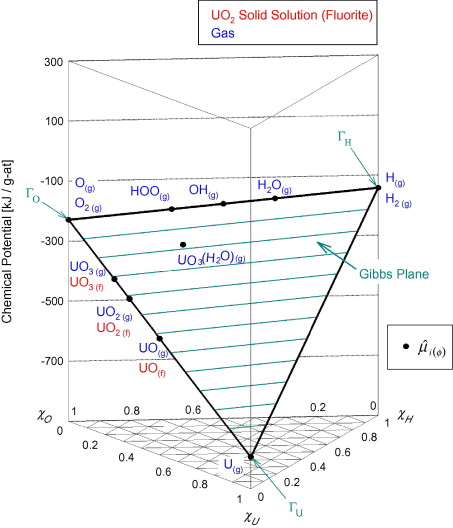
\includegraphics[width=0.52\textwidth]{figures/Gibbs_plane.jpg}
		\caption{The Gibbs criteria is satisfied when the chemical potentials for all species represented per gram-atom lie on the Gibbs Plane within an acceptable tolerance \cite{Piro11a}.}
		\label{fig:GibbsPlane}
	\end{figure}

	The chemical potential of any point on the Gibbs plane can be expressed as a linear combination of  chemical potentials of system components and this interpolated potential can be denoted by $\hat{\mu}_{i(\phi)}(\Gamma)$. The absolute difference between $\hat{\mu}_{i(\phi)}(\Gamma)$ and $\hat{\mu}_{i(\phi)}$, $\Psi_{\Gamma}$ can then be used as convergence criterion:
		\begin{equation}\label{eqn:convGC}
			\Psi_{\Gamma} = \left \vert  \hat{\mu}_{i(\phi)}(\Gamma) - \hat{\mu}_{i(\phi)} \right \vert < \epsilon
		\end{equation}
	 i.e., all the species in equilibrium must lie on the Gibbs plane. If a phase lies below the Gibbs plane, adding it to the phase assemblage would yield a lower Gibbs energy of the system and such a system would not be at a global minimum. The Gibbs criteria is easily extendable to electrochemical equilibrium and can be conveniently implemented in a thermodynamic equilibrium	 solver.

	\section{Global optimisation}\label{sec:global_opt_intro}
	 Global minimisation of Gibbs energy is crucial to accurately predicting the stable phase assemblage using equilibrium thermodynamic softwares. An example application is the detection of miscibility gaps in phases containing regions of compositional instability. In a miscibility gap, the same phase can appear with different compositions and finding the global minimum from among the many local minima can be a daunting challenge. For multi-component systems, the topology of the energy surfaces tends to become quite complex particularly when there are multiple non-ideal phases in the system. This significantly complicates the interaction of the Gibbs energy surface with the Gibbs hyperplane and an inadequate numerical approach may lead to a false sense of thermodynamic equilibrium despite being far from the true equilibrium. To illustrate how an inadequate solver may yield a false equilibrium, the following scenarios can be considered:
	\begin{enumerate}
		\item In the fictive binary system shown in figure~\ref{fig:go_sys-AB}, a solution phase $\alpha$ and a stoichiometric phase \ce{A3B2} can possibly coexist. While the stoichiometric phase \ce{A3B2} and solution phase $\alpha$ are predicted to be stable, as represented by the dashed tangent line, they are in fact metastable and a miscibility gap would yield a lower value of the integral Gibbs energy of the system, $G_\text{sys}$.
		\begin{figure}[htbp]
		\centering
		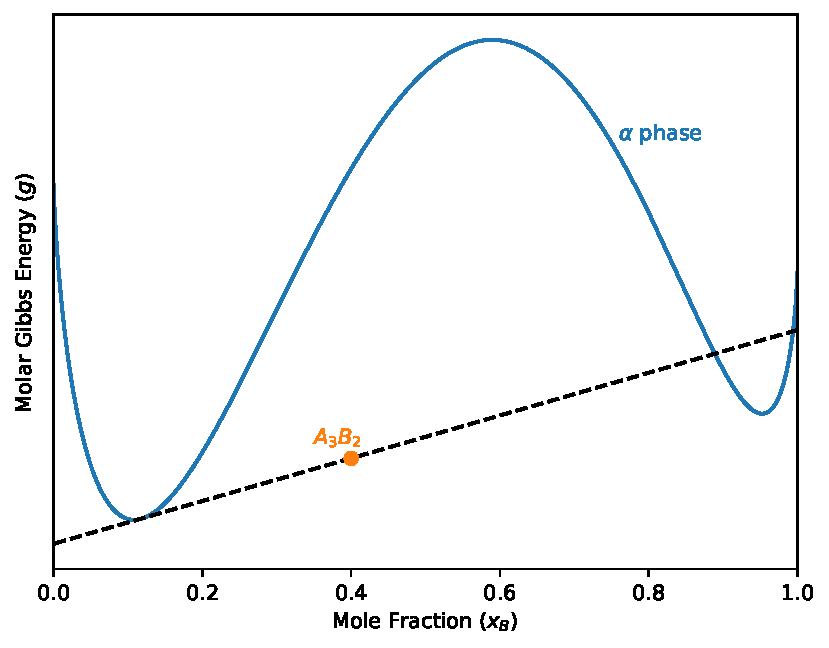
\includegraphics[width=0.75\textwidth]{figures/chapter-4/System_AB.pdf}
		\caption{Fictive system with miscibility gap showing a possible false positive from thermodynamic equilibrium solver (after Piro and Simunovic \cite{Piro16}).}
		\label{fig:go_sys-AB}
	\end{figure}

	\item In the fictive binary system shown in figure~\ref{fig:go_sys-CD} which can have three possible solution phases, the $\delta$ phase is believed to be metastable but one must confirm that the combination of $\beta$ and $\gamma$ is most stable or if a different combination is more stable. However, it can be seen that inserting the $\delta$ phase into the system and replacing one of the other two phases would yield a lower value of the integral Gibbs energy of the system, $G_\text{sys}$.
		\begin{figure}[htbp]
		\centering
		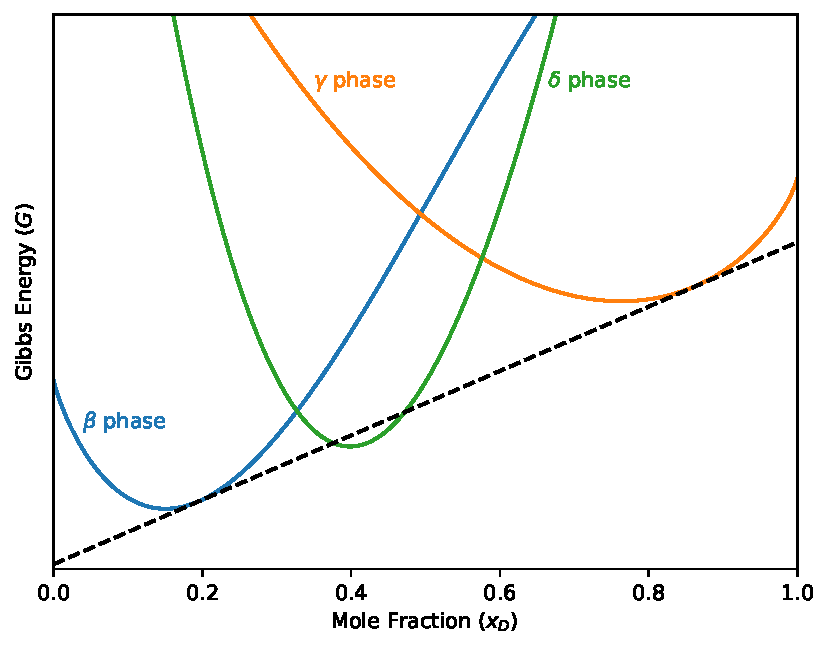
\includegraphics[width=0.75\textwidth]{figures/chapter-4/System_CD.pdf}
		\caption{Fictive system with three possible phases showing a false positive from thermodynamic equilibrium solver wherein a wrong phase is believed to be present at equilibrium (after Piro and Simunovic \cite{Piro16}).}
		\label{fig:go_sys-CD}
	\end{figure}
	\end{enumerate}





\section{Summary of Thermodynamic Equilibrium}
Achieving thermochemical equilibrium in a system requires satisfaction of several conditions which are as follows:
	\subsection{Necessary conditions}
    	\begin{enumerate}\compresslist
        		\item \emph{Conservation of mass} requires that the mass of element $j$, $b_j$, must satisfy the following mass balance equation
            	\begin{equation}
                		b_j = \sum_{\lambda=1}^{\Lambda} n_{\lambda}\sum_{i=1}^{N_{\lambda}}x_{i({\lambda})}{\nu}_{i,j} +  \sum_{\omega=1}^{\Omega} n_{\omega}{\nu}_{\omega}
            	\end{equation}
            	where, ${\nu}_{i,j}$ and ${\nu}_{\omega}$ represent the stoichiometric coefficients of element $j$ in solution phase species $j$ and stoichiometric phase $\omega$ respectively.
        		\item \emph{Gibbs' phase rule} which defines the thermodynamic degrees of freedom of the system must also be     satisfied
            	\begin{equation}
                		F=C-\Phi + 2 + \Xi
            	\end{equation}
            	where, $F$ represents the degrees of freedom, $C$ denotes the number of components in the system, $\Phi$ denotes the number of phases and $\Xi$ denotes the number of ionic phases.
        		\item \emph{Gibbs' criteria} for equilibrium requires that the Gibbs energy of a system be at a global equilibrium. In equivalent terms, the chemical potential for each system component must have the same value in all stable phases within the system \cite{HILLERT198131}, where the chemical potential of any constituent in a stable phase can be defined as a linear function of the element potentials, $\Gamma_j$, as
            	\begin{equation}
		        \mu_{i} = \sum_{j=1}^C \nu_{i,j} \Gamma_j
            	\end{equation}
    	\end{enumerate}

	\subsection{Sufficient conditions}
    	The necessary conditions for thermodynamic equilibrium require that the chemical potentials of all stable solution phase species and stoichiometric phases abide by the above equality, which is equivalent to Gibbs energy of the system being at a local minimum, and that the conservation of mass and the Gibbs phase rule are satisfied. The sufficient condition requires that all the metastable phases abide by the following conditions
    	\begin{equation*}
        		\pi_{\lambda} = \min_{\lambda} \sum_{i=1}^{N_{\lambda}}x_{i({\lambda})} \left (\mu_{i({\lambda})} - \sum_{j=1}^C \nu_{i,j}\Gamma_j \right )
    	\end{equation*}
    	i.e., there must exist a Gibbs' plane such that the element potentials lie on the plane and the chemical potentials of all the species lie on or above the plane and the mole fraction of the species must satisfy the following constraints
	\begin{equation}
        		\begin{aligned}
            		\sum_{i=1}^{N_{\lambda}}x_{i({\lambda})} = 1 \\
			x_{i({\lambda})} \geq 0 \;\; \forall i
        		\end{aligned}
    	\end{equation}
    	i.e., the sum of mole fraction of all the species in a phase $\lambda$ must be unity and that the individual mole fractions must be greater than or equal to zero.

    	The aforementioned conditions are used in Gibbs energy minimisers to find a unique combination of phases that are stable in the system.
